\documentclass[conference]{IEEEtran}
\IEEEoverridecommandlockouts
% The preceding line is only needed to identify funding in the first footnote. If that is unneeded, please comment it out.
\usepackage{cite}
\usepackage{amsmath,amssymb,amsfonts}
\usepackage{algorithmic}
\usepackage{graphicx}
\usepackage{textcomp}
\usepackage{xcolor}
\usepackage{adjustbox}
\usepackage{array}
\usepackage{float}
\usepackage{graphicx}
\usepackage{longtable}

\def\BibTeX{{\rm B\kern-.05em{\sc i\kern-.025em b}\kern-.08em
    T\kern-.1667em\lower.7ex\hbox{E}\kern-.125emX}}
\begin{document}

\title{FourGuys proposal to further improve the point-of-sale system: Checkout\\}

\author{\IEEEauthorblockN{Sven Veit}
\IEEEauthorblockA{\textit{dept. of Economics} \\
\textit{Kiel University of Applied Sciences}\\
Kiel, Germany\\
svenveit@hanyang.ac.kr}

\and
\IEEEauthorblockN{Jiyong Lee}
\IEEEauthorblockA{\textit{dept. of Educational Technology} \\
\textit{Hanyang University}\\
Seoul, Korea\\
jdragon2000@naver.com}

\and
\IEEEauthorblockN{Zabolotniaia Anna}
\IEEEauthorblockA{\textit{dept.Business Administration} \\
\textit{Hanyang University)}\\
Seoul, South Korea\\
elijaltayer@gmail.com}

\and
\IEEEauthorblockN{Aneesa Shaki}
\IEEEauthorblockA{\textit{dept. of Engineering and Computer Science} \\
\textit{University of New South Wales}\\
Sydney, Australia\\
a.shaki@student.unsw.edu.au}
}

\maketitle

\begin{abstract}
 This document will define our proposal requirements, and explain our motivations and ongoing roles throughout the initial development process of the project and fulfil client requirements with an application to improve the POS system. This project aims to develop an enhanced POS (Point of Sale) system that leverages smartphone-based barcode scanning technology to enable customers to complete their purchases without the need to wait in checkout lines. By using our mobile application, users can simply scan product barcodes as they shop, automatically adding items to a virtual shopping cart. When ready, they can complete the payment through the app’s secure and user-friendly interface, eliminating the need for traditional cashier interactions. This system not only reduces customer wait times but also minimizes staff workload and enhances the shopping experience by providing a seamless and efficient checkout process. 
\end{abstract}

\begin{IEEEkeywords}
POS system, barcode scanning, mobile payment, contactless checkout
\end{IEEEkeywords}

\section{Introduction}

\subsection{Motivation}
Amid the ongoing cost of living crisis and the rapid shift in consumer behavior, large retailers are increasingly focused on improving operational efficiency and cutting costs to meet rising customer expectations. Recent disruptions, including global supply chain issues and changing labor dynamics, have amplified the urgency for more innovative, cost-effective solutions in the retail industry. While technological advancements have already revolutionized the checkout process, most notably with the introduction of contactless kiosks as the benchmark for modern Point of Sale (POS) systems, there is still untapped potential for further improvement. \\
By capitalizing on the most universally accessible tool, the smartphone, we have the opportunity to not only reduce costs but also redefine the customer experience. The current retail landscape demands flexibility, and utilizing smartphones as mobile POS systems is a natural progression. This approach can significantly reduce infrastructure costs, eliminate the need for fixed kiosks, and decrease reliance on labor-intensive processes. Existing solutions allow QR and barcode scanning, but this project goes beyond that, aiming to fully integrate smart devices into the shopping journey. By empowering consumers to scan and purchase items independently, we can deliver a frictionless, personalized retail experience that meets the evolving demands of today's shoppers, while future-proofing retail operations against future disruptions 

\subsection{Problem Statement}
The current issues within the economy due to the current inflation globally has caused for a need to reduce costs within the retail industry to place less burden on the consumer with a lack of leeway within produce and goods adaptations to the current POS systems and how to increase the efficiency and costs for the business whilst simplifying the process for the consumer are concerns of leading industry giants. \\

The main issues are as follows: \\
\subsubsection{Long wait times and congestion}

After completing their shopping, customers often face long queues at the checkout, especially during peak hours. This not only causes discomfort for customers, but also forces stores to operate more checkout counters or hire additional staff to maintain efficiency. These measures lead to increased costs and reduced customer satisfaction. 

\subsubsection{Increased costs}
Installing and maintaining traditional POS systems and kiosks incurs significant costs, which rise exponentially as the size of the store increases. Additionally, these systems require regular updates and maintenance, further driving up operational expenses.

\subsubsection{Lack of flexibility}
The current payment system relies on fixed checkout counters or kiosks, which makes it difficult to adapt to customer traffic flow or shopping patterns. This limitation hampers the store's ability to manage in-store congestion or offer more convenient options to customers.

\subsubsection{Limited customer experience}
Current payment systems do not provide customers with enough control over their shopping experience, such as real-time price checking or managing their shopping list. This limits customers' ability to self-manage information related to their purchases. \\

These issues lead to customer dissatisfaction and increase operational costs. Our project aims to address these problems by introducing a mobile-based payment system that increases efficiency, reduces costs and improves the customer experience by allowing a streamlined seamless method of payment. 

\subsection{Solution}
Our proposal is to solve this current problem through a mobile application that has the capabilities of functioning as a POS system within physical retails stores. 

With this solution, customers can avoid traditional checkout lines, significantly reducing congestion and wait times, especially during peak shopping hours. Since there is no need for physical POS kiosks or additional staff assistance, retailers can drastically lower their infrastructure and labour costs. Moreover, this system allows retailers to move beyond the limitations of fixed checkout counters, adapting more flexibly to fluctuating customer flows. 

Using smartphones also empowers customers to have more control over their shopping experience. They can access real-time information on prices, promotions, and their total cart value, easily add or remove items, and apply discounts automatically, completing transactions without physical interaction. This enhances convenience and safety, especially in the post-pandemic era where contactless solutions are highly valued. 

By integrating this mobile-based payment system, we aim to not only boost operational efficiency but also transform the overall shopping experience into a more flexible, cost-effective, and customer-centric retail environment. 

\subsection{Related Software}

\subsubsection{Amazon Price Comparison and Product Scanner}
Amazon’s mobile app allows users to scan product barcodes and instantly access product information, reviews, and pricing within Amazon’s marketplace. Available on both iOS and Android, this app uses barcode scanning to retrieve product details, enabling users to compare Amazon’s prices with in-store prices. This functionality closely aligns with the goals of our project.

\subsubsection{ShopSavvy Barcode Scanner}
ShopSavvy is an app that allows users to scan barcodes to view pricing and availability across various online and local stores. Available on the App Store and Google Play Store, ShopSavvy’s barcode scanning technology and its price comparison feature across multiple retailers align closely with the objectives of our app.

\subsubsection{Google Lens}
Google Lens can scan barcodes and provide detailed product information, including prices, from various online sources. Integrated within Google Search and Google Photos, Google Lens uses advanced image recognition and search capabilities to retrieve product information via barcodes, which mirrors the core functionality of our proposed app.

\subsubsection{Barcode Scanner Algorithm}
Algorithms like ZBar and pyzbar are widely used in Python for barcode detection and decoding in various apps and services. The pyzbar Python library, available at https://pypi.org/project/pyzbar/, offers an open-source solution for reading barcodes in images, making it a potential foundational component for implementing the barcode scanning functionality in our app.\\

\subsection{Smart Trolleys}
Smart Trolleys are advanced shopping carts equipped with technology such as touchscreens, barcode scanners, and weight sensors to enhance the in-store shopping experience. Currently being trialed by some stores, these trolleys allow customers to scan and bag items as they shop, track spending in real time, and receive personalized offers or recommendations. They aim to streamline the checkout process, reduce wait times, and provide a more interactive and efficient shopping journey.


These references illustrate existing solutions and technologies that provide similar barcode
scanning and price comparison features. For our app, integrating similar barcode decoding
libraries and developing a comparison feature across supermarkets would differentiate it by
focusing on price comparisons specifically within the grocery retail sector


\subsection{Role Assignments}
\begin{table}[H]
    \centering
    \caption{Role Assignments}
    \begin{adjustbox}{max width=\textwidth}
        \begin{tabular}{|>{\centering\arraybackslash}m{1.2cm}|>{\centering\arraybackslash}m{1.2cm}|m{5cm}|}
            \hline
            \textbf{ Role} & \textbf{ Name} & \textbf{ Task} \\
            \hline
            Software Developer & Sven & Responsible for designing, implementing, and maintaining scalable backend systems while overseeing technical decision-making and ensuring high-quality code across all projects. Defines backend architecture, mentors the development team, enforces coding standards, and manages system performance, security, and reliability. Collaborates with stakeholders, guides Agile workflows, adopts emerging technologies, and drives innovation to deliver robust, maintainable software. \\
            \hline
            Software Developer & Aneesa &Contributes to the development and maintenance of backend systems using JavaScript/Node.js while assisting in creating and managing technical documentation. Supports the implementation of APIs, database interactions, and backend logic to ensure robust and efficient functionality. Assists in documenting system architecture, APIs, workflows, and best practices to maintain clarity and alignment across teams. Collaborates with team members to troubleshoot issues, improve code quality, and streamline development processes while ensuring all technical documentation is up-to-date and accessible. \\
            \hline
            Front-end Developer & Jiyong & Develops and optimizes user interfaces (UI) for web and mobile applications, ensuring a seamless and responsive user experience (UX). Collaborates with designers to implement visually engaging and accessible components, focusing on usability and interactivity.
            Ensures cross-platform compatibility and addresses performance optimization for efficient rendering and responsiveness.\\
            \hline
            Graphics Designer & Anna & To construct a visual design for the user experience  \\
            \hline
        \end{tabular}
    \end{adjustbox}
\end{table}

\section{Requirements}

\subsection{Barcode Scanner Feature}
\subsubsection{Barcode Scanning via Camera}
Users can scan product barcodes using their smartphone camera, enabled by the QuaggaJS library, which decodes barcodes from video streams in real time. JavaScript's navigator.mediaDevices.getUserMedia() API streams the camera feed to the browser, allowing the library to process frames and detect barcodes. Once detected, a backend API (built with Node.js) fetches detailed product information, including descriptions, prices, and availability, and updates the UI dynamically via frameworks like React.js or Vue.js.
\subsubsection{QR Code Scanning Support}
 QR code functionality is achieved using libraries like html5-qrcode or qrcode.js, which decode QR codes in the browser. JavaScript captures the camera feed, and when a QR code is scanned, the encoded data is processed to apply promotions or fetch additional product information. This real-time update mechanism ensures the discounts and offers are reflected in the shopping cart without manual intervention, enhancing user convenience.
\subsection{Shopping Cart Feature}
\subsubsection{Add Products}
When users scan a product barcode, product details fetched from an API are added to a state-managed shopping cart using tools like Redux or Vuex. JavaScript functions dynamically update the cart, showing item details like name, price, and quantity in real time, while re-rendering the cart component for seamless user interaction.
\subsubsection{Modify and Remove Products}
Event listeners are implemented in buttons or input fields for quantity adjustments or product removal. These actions trigger JavaScript functions that update the cart state, recalculating totals dynamically using helper functions. The updated state is rendered immediately to provide users with an accurate overview of their cart.
\subsubsection{View Total Payment Amount}
JavaScript calculates the cart total, including taxes and discounts, using array manipulation methods like reduce() to iterate over the cart items. Real-time updates ensure that any changes to the cart, such as adding a product or applying a discount, are reflected instantly. The calculated total is displayed in the shopping cart summary, helping users monitor their expenses.
\subsection{Payment Feature}
\subsubsection{Choose Payment Methods}
Users can register multiple payment methods, securely stored as tokens using the Stripe.js library. JavaScript interfaces enable adding, editing, or deleting payment methods, with seamless updates to the user’s profile managed through API calls.
\subsubsection{Instant Payment}
The app leverages Stripe’s JavaScript SDK to securely capture payment details and process transactions with minimal latency. A “Pay Now” button triggers an API call to Stripe, ensuring secure payment processing through tokenized data. Real-time status updates are provided on the frontend using JavaScript promises or async/await.
\subsubsection{View Payment History}
JavaScript fetches transaction data from a backend database using REST APIs and displays it on the user’s profile page. Libraries like React Query facilitate efficient fetching, caching, and displaying of itemized receipts, enabling users to review their past orders and spending history conveniently.
\subsection{Promotions and Coupon Management}
\subsubsection{Register Discount Codes/Coupons}
Users input discount codes through a form validated by JavaScript, which verifies the code's format and validity via an API call. Valid codes are stored in the user’s profile, and JavaScript applies them automatically to eligible purchases during checkout, reflected in real-time cart updates.
\subsubsection{Automatic Coupon Application}
During product scanning, the system checks against a database of active promotions via API integration. JavaScript automatically applies applicable discounts, using updated cart states to display reduced prices without requiring user input.
\subsubsection{Reward Programs}
Rewards are tracked through a points system, updated using backend APIs and displayed in the frontend with JavaScript. Users can view their rewards and redeem points during checkout, with real-time deductions and updates managed by JavaScript functions interacting with the backend.
\subsection{Notifications and Push Features}
\subsubsection{Promotion Notifications}
JavaScript integrates with push notification services like Firebase Cloud Messaging (FCM) to send real-time alerts about discounts and special offers. Users customize notification settings through a frontend interface, saved using JavaScript and synced with the backend.
\subsubsection{Payment and Order Notifications}
Upon payment completion, JavaScript triggers notifications using WebSocket-based libraries like Socket.IO, ensuring immediate updates. These notifications inform users of payment success, order confirmations, and shipping status.

\subsection{User Profile Management}
\subsubsection{Manage Personal Information}
JavaScript captures user input for profile updates, validates the data using libraries like Yup, and sends it to the backend via API calls. Changes are reflected immediately on the frontend, providing users with an updated and secure experience.
\subsubsection{Manage Payment Information}
JavaScript handles adding and editing payment methods securely via the Stripe.js library. Users interact with a dynamic interface built with frameworks like React, ensuring smooth updates to payment preferences stored on the server through tokenized API interactions.



\section{Development Environment}
\subsection{Development Platform}
Web application platform is suitable for our software due to its accessibility, scalability and cross platform compatibility. Unlike traditional desktop applications, a web application can be accessed from any device with internet access, allowing users to interact with the software in real time without requiring specific hardware or operating system configurations. This flexibility significantly broadens the user base, as it eliminates the need for installations or updates on individual devices. Additionally, web applications are naturally scalable, making it easy to accommodate growing user demands and adapt to changing requirements with no requirement to accommodate to the OS system of a device reducing the complexity of the project. Development frameworks for web applications also offer extensive libraries and tools that accelerate development and provide built-in security features, which are crucial for protecting sensitive data. Altogether, these advantages make a web application an optimal platform for delivering robust, user-friendly, and secure software solutions.  

\subsection{Coding Langauges}
\subsubsection{Javascript}
JavaScript is a coding language influenced by Java with syntax derived from C.  
It is enriched by a vast ecosystem of libraries and frameworks that enhance its capabilities in barcode scanning, data handling, and API integration. Libraries like QuaggaJS, jsBarcode, and Dynamsoft are specifically designed for barcode scanning, enabling web applications to process barcode data directly through the browser. For data handling, libraries such as Lodash and D3.js offer powerful tools for data manipulation, visualization, and transformation, making it easier to process large datasets and present them in interactive, user-friendly formats. 
JavaScript also offers comprehensive support for API integration, with libraries like Axios and Fetch simplifying asynchronous data requests and responses. For handling real-time data, libraries such as Socket.IO facilitate WebSocket connections, allowing developers to create applications that update dynamically without page reloads. Additionally, popular frameworks like React, Angular, and Vue streamline the development of user interfaces, providing reusable component architectures and state management tools, while libraries such as jQuery simplify DOM manipulation and event handling. These frameworks and libraries, along with JavaScript’s cross-platform support, make it an essential language for building feature-rich, responsive, and data-driven web applications.Compatible software development frameworks include Node.js and React Native which offer an extensive library for building and developing software and a range of tools.  

\subsubsection{Typescript}
Typescript is an extension of JavaScript that implements static typing, classes and interfaces. This allows for optimal code organisation and object-oriented programming techniques. Typescript allows for improved error detection with additional tooling support that enhances the IDE experience and ensures proper API documentation. 

\subsubsection{CSS}
CSS frameworks and libraries complement JavaScript, offering pre-designed, responsive UI components that enhance the styling and layout of web applications. Libraries like Bootstrap, Tailwind CSS, and Bulma streamline styling by providing ready-made classes for layouts, typography, buttons, and more, allowing developers to quickly achieve consistent, visually appealing designs. Additionally, CSS animation libraries, like Animate.css and GreenSock (GSAP), enable smooth transitions and dynamic visual effects that bring interactivity to user interfaces. 

\subsubsection{HTML}
HTML is the core language for structuring and presenting content on the web. It serves as the foundation of web pages, defining elements like headings, paragraphs, images, links, and forms, enabling browsers to interpret and display content in a coherent layout. The latest version, HTML5, introduced new semantic tags such as header, footer, article, and section, which help organize content more meaningfully while improving accessibility and search engine optimization (SEO). HTML5 also brought powerful features for embedding multimedia through audio and video elements, along with APIs that enable functionalities like local data storage and geolocation, enhancing interactivity and user experience in web applications. Working together with CSS for styling and JavaScript for interactivity, HTML is essential for building accessible, structured, and user-friendly websites and applications. 

\subsection{Cost Estimation}
\begin{table}[H]
    \centering
    \caption{Cost Estimation Table}
    \begin{adjustbox}{max width=\textwidth}
        \begin{tabular}{|>{\centering\arraybackslash}m{1.8cm}|>{\centering\arraybackslash}m{1.2cm}|m{4.6cm}|}
            \hline
            \textbf{ Expense attribute } & \textbf{ Cost per annum } & \textbf{ reasoning } \\
            \hline
           Web Hosting and Server Costs  & \$1200-2400  & Platforms such as AWS, Google Cloud or Heroku are required to host the website for use to deliver reliable, scalable and high-performance solutions.  \\
            \hline
            Database Hosting  & \$240-600  & Database hosting provides infrastructure needed to store, manage and access databases over the internet. Examples of database host include Firebase, MongoDB Atlas or MySQL.  \\
            \hline
            Outsourced API  & \$600-1200  & In the case of using a third party API to access barcode scanning libraries to reduce code development and focus on the websites functionalities.  \\
            \hline
            Domain Name/registration  & \$0-20  & The costs associated to secure a domain name.   \\
            \hline
            SSL  & \$0-249  & A digital authentication of the websites identity and enables encrypted connection for security purposes and needed to accept online payments.   \\
            \hline
        \end{tabular}
    \end{adjustbox}
\end{table}

\subsection{Software in Use}
\subsubsection{VSCode}
VSCode (Visual Studio Code) is our chosen code editor due to its flexibility and extensive support for various programming languages and extensions. It plays an important role in our project, which involves creating an application that allows users to scan barcodes with their phones for payment. VSCode allows us to customize our workspace and integrates well with Git, enabling us to efficiently track code changes. Additionally, it provides features like live sharing and remote development, enhancing collaboration and productivity among team members. 

\subsubsection{Gitlab}
Git serves as our core version control system, essential for tracking and managing code changes systematically. GitLab complements Git by providing a self-hosted platform with robust DevOps tools, allowing us to manage our barcode payment app project in one integrated environment. GitLab’s CI/CD (Continuous Integration and Continuous Deployment) features are especially valuable for automating testing and deployment processes, which helps streamline our development pipeline. It also offers comprehensive project management tools, enabling us to oversee the entire lifecycle of the project in one place, from issue tracking to deployment. GitLab’s integrated approach enhances our ability to handle tasks efficiently and keep the development process organized. 

\subsubsection{Github}
While GitLab serves as our primary development platform, GitHub complements our workflow by providing a strong collaborative environment for code review and open-source visibility. GitHub’s large community and social coding features, such as pull requests, make it ideal for reviewing and managing contributions from multiple team members. GitHub's user-friendly interface and extensive integrations also make it an excellent choice for code sharing and feedback. Unlike GitLab, which focuses heavily on integrated DevOps workflows, GitHub excels in fostering collaboration and is widely used by developers for code management. By using GitHub, we ensure code quality and organization, which aligns well with our project’s focus on creating a robust barcode payment app. 

\section{Specifications}

\subsection{Login page}
The login feature allows users to access their payment methods and purchase history. Upon entering a valid username and password, and pressing the login button, a login POST API request is sent to the server for authentication. For enhanced security, passwords are stored using encryption methods like hashing and salting. In case of multiple failed login attempts, additional security measures such as CAPTCHA or account lockout mechanisms may be implemented.

\subsection{Register page}
 The email address must be a valid, unique email, serving as the user’s primary identifier for login and communication. The password must be a combination of English letters and numbers, with a length between 8 and 15 characters, and may optionally include special characters to enhance security. During registration, the system ensures the email is not already associated with an existing account, maintaining uniqueness. Once registration is complete, the user’s email and password are securely stored in the database using industry-standard encryption methods to protect sensitive information.
 
 \subsection{User information page}
 On the update their personal information which will provide them access to ensure the safety of their account and view their current email address or update their password if required. The use information page will also provide access to personal information relevant to the application including credit card information, help services for the application or payment data.
 
 \subsection{Card Payment}
On the payment page, users can securely complete their transactions through a trusted third-party service, such as Stripe. When a payment is made, the user is directed to Stripe’s payment gateway, which handles the processing of card or account details. Users can select from previously registered payment methods or add a new one during the transaction. Stripe ensures the payment request is securely processed, sending approval or rejection responses back to the app.
Sensitive payment information, such as card details, is not stored in the app’s database but is securely tokenized and managed by Stripe, adhering to industry standards for encryption and data protection. For added security, login sessions and API requests are fortified to prevent unauthorized access. Users can also access their purchase history within the app to view past transactions. This history, linked to the payment service, can be used to recommend items of interest or provide easy access to receipts and transaction details.

\subsection{Barcode scanning page}
The application should be able to effectively scan store barcodes to add the product to the customers card to allow them to complete a purchase. Once camera access has been permitted by the user the application should have access to the store database to adjust the quantity of the sock and accurate provide the price, quantity or amount and description of product to the cart.

\subsection{Shopping Cart and Checkout}
Users will be able to add, modify, or remove items in their shopping cart with ease. The checkout process will be streamlined, offering multiple payment options, including credit cards, digital wallets, and payment through services like Stripe or PayPal. Features like order summaries, tax calculations, and discount codes will be integrated for a seamless transaction experience.

\subsection{Payment Gateway Integration}
A trusted third-party payment gateway, such as Stripe, will be integrated to handle secure transactions. The payment system will support various payment methods and currencies to accommodate diverse user needs. Tokenization and encryption will ensure sensitive data is protected, with compliance to industry standards like PCI DSS.

\subsection{Order Management and Notifications}
The application will allow users to track their orders in real-time, with automated notifications sent for order confirmation, shipping updates, and delivery status. The system will integrate with delivery services for accurate tracking and provide an option for users to manage returns or report issues.

\subsection{Admin Dashboard}
An admin interface will enable store managers to upload and manage products, monitor inventory, review sales reports, and process refunds or returns. Analytics tools will provide insights into user behaviour, sales trends, and marketing performance to optimize business strategies.


\subsection{Reviews and Ratings}
Customers will be able to leave reviews and rate products, helping to build trust and provide valuable feedback for other users. A moderation system will ensure reviews meet community guidelines, while highlighting top-rated products to enhance visibility.

\subsection{Cross-Platform Compatibility}
The application will be developed to function seamlessly on web and mobile platforms, ensuring a consistent user experience across devices. Responsive design principles will optimize the interface for various screen sizes, while dedicated mobile apps for iOS and Android will provide enhanced functionality for mobile users.

\subsection{Security and Data Privacy}
The application will prioritize security with encryption protocols, secure APIs, and regular vulnerability assessments. Compliance with data privacy regulations, such as GDPR or CCPA, will be maintained to safeguard user information and build trust.

\subsection{Scalability and Maintenance}
The platform will be designed to accommodate future growth, with a scalable architecture that can handle increased traffic and new features. A maintenance plan will include regular updates, bug fixes, and customer support to ensure the application remains reliable and up to date.

\section{Architecture Design and Implementation}

\subsection{Overall architecture}
Below is the system architecture design for our application, which will be deployed on 
Microsoft Azure Cloud. The architecture is modular, with clear relationships and 
functionality between components. The design incorporates frontend, backend, 
database, external services, and Azure cloud features. 

\subsubsection{Frontend}
Description: This module allows users to interact with the application via a web-based 
interface. 
Required Classes: - - - 
`BarcodeScanner` (for scanning barcodes) 
`PaymentGatewayUI` (for processing payments) 
`ReceiptViewer` (for displaying receipts) 
Technologies: HTML, CSS, JavaScript, Node.js, SQL 
\subsubsection{API Gateway }
Description: Acts as the bridge between the frontend and backend, handling all API 
requests and responses. 
Required Classes: - - 
`RequestHandler` (handles API calls from the frontend) 
`Authenticator` (validates user requests) 
Technologies: Node.js with Express.js 
\subsubsection{Backend}
Description: Processes all requests, retrieves data, handles business logic, and 
communicates with external APIs and the database. 
Required Classes: - - - 
`ProductManager` (fetches product information from the database) 
`PaymentProcessor` (handles payment transactions) 
`ReceiptHandler` (stores and retrieves receipt data) 
Technologies: Node.js, Express.js 
\subsubsection{Database}
Description: Stores product data, user data, receipts, and store details. 
Required Classes: - - - 
`ProductsTable` (product details like barcode, price, and name) 
`ReceiptsTable` (stores completed transactions) 
`StoresTable` (location-based store details) 
Technologies: Azure SQL Database 
\subsubsection{Azure Cloud Services}
Description: Hosts the application and provides additional cloud services for scalability 
and reliability. 
Components: - - - - 
Azure App Service: Hosts the frontend and backend. 
Azure SQL Database: Stores all structured data. 
Azure Blob Storage: For storing assets like receipts, images or JSON files. 
Azure Key Vault: Manages sensitive information like API keys securely. 
\subsubsection{Third-Party Services}
Description: Integrates external APIs and libraries for specific functionalities such as 
payment processing. 
Required Components: - - 
JavaScript Barcode Library: Used directly within the frontend for barcode 
scanning. No external API is required. 
Payment Gateway API: For processing payments (e.g., Stripe, PayPal).

\begin{figure}[H]  % 'h'는 이미지가 해당 위치에 삽입되도록 지정
    \centering  % 이미지를 중앙에 배치
    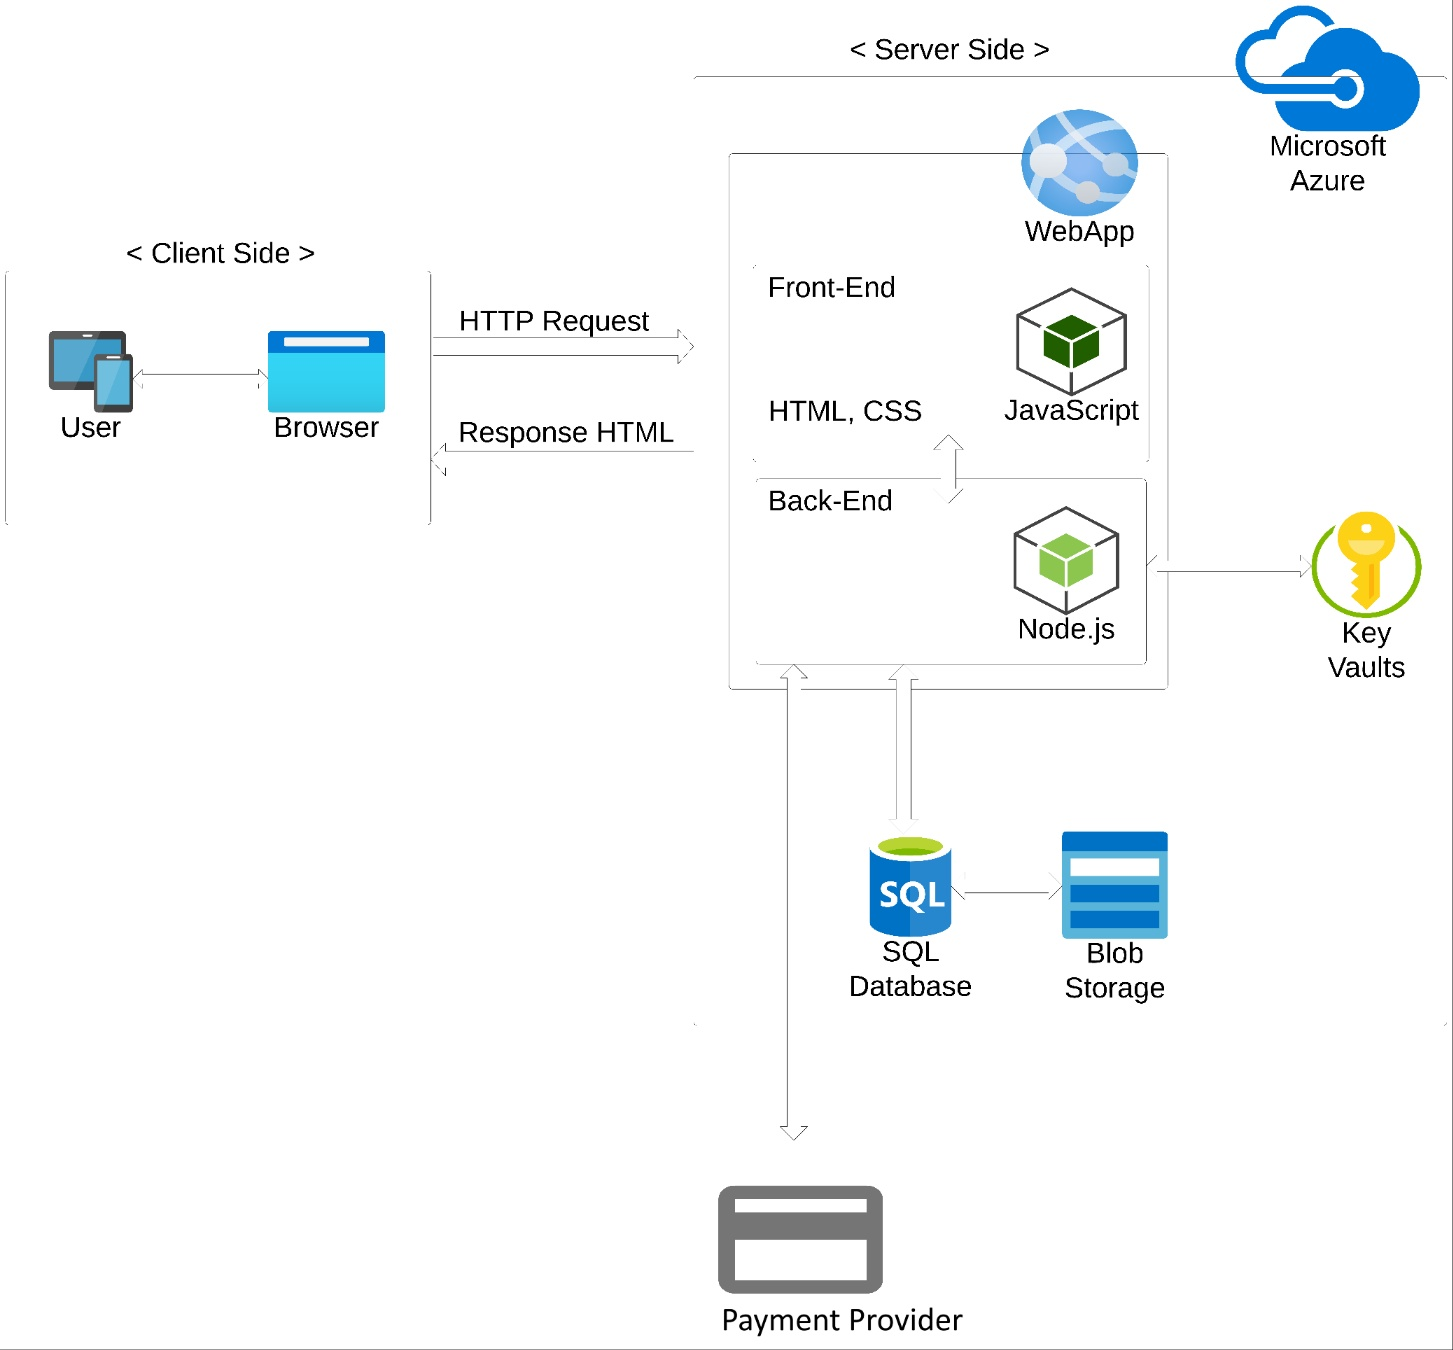
\includegraphics[width=0.5\textwidth]{architecture.jpg}  % 이미지 크기와 파일명 지정
    \caption{Overall Architecture}  % 이미지 캡션
\end{figure}

\subsection{Directory organization}

\begin{itemize}
  \item Undefined/Success.html : This HTML page confirms a successful payment and interacts with a backend API to generate a receipt. It includes a header displaying a success message, and a footer with navigation links (home, scanner, receipts, cart, account). The script checks if the user is logged in by retrieving the user ID from localStorage. If not, it prompts the user to log in. After confirming payment, a POST request is sent to the backend API with the user ID in the headers. If the request is successful, a receipt is generated; otherwise, an error message is shown. The page is designed to be responsive and includes external CSS for styling.
  \item Undefined/Style.css: Provides a responsive, user-friendly design for a website, covering authentication, shopping, scanning, receipts, cart, account settings, and footer navigation. It resets default margin and padding for consistency, styles the body with a clean background, and centers the header. The authentication section includes a login button with hover effects. Shop and bookmark items are displayed using flexbox with hover effects. The scanner section is responsive, ensuring the video fits its container. Receipts and cart sections feature interactive list items with product details and removal options. Account settings offer action and logout buttons, with distinct hover effects. The footer navigation is fixed at the bottom, with icons that change color on hover. Media queries ensure responsiveness across devices, enhancing both functionality and appearance.
  
  \item Undefined/Stripe.html: Sets up a basic Stripe payment flow. It includes a header with a title, a button for triggering the payment process, and a footer with navigation links represented by icons for home, scanner, receipts, cart, and account pages. The JavaScript embedded in the page handles the payment logic by listening for a click on the "Pay Now" button. Upon clicking, it first checks if the user is logged in by retrieving the user ID from localStorage. It then fetches the user's cart data from a backend server and ensures the cart contains items. Afterward, it communicates with the backend to create a Stripe checkout session and redirects the user to Stripe's hosted payment page. If any errors occur during the process, relevant error messages are displayed, ensuring a smooth user experience.
  \item Undefined/Receipts.html: This HTML code displays a user's receipts. It includes a header with a title, a section for listing receipts dynamically injected into the page, and a footer with navigation links to other sections (home, scanner, receipts, cart, and account). The JavaScript manages the display of receipts by first checking if the user is logged in (using localStorage to retrieve the user ID). It then fetches receipt data from a backend server and populates the receipt list. Each receipt displays details like purchase date, total sum, and shop name, with an option to delete receipts. When clicked, each receipt can expand to show more details about the items purchased. If no receipts are available, a message is shown. The user can also delete receipts, and the list is reloaded after a successful deletion. If any errors occur during data fetching or deletion, relevant messages are displayed.
  \item Undefined/Index.html: This HTML page represents the home screen of an application, where users can view available shops and manage bookmarks. Upon visiting the page, the script checks for a valid user session through a stored ID token and displays user-specific information. The main content of the page consists of a list of shops, from which users can select a shop, and a list of product bookmarks with options to remove items from the list. The JavaScript first handles login redirects, storing user information in localStorage and updating the UI with a welcome message. The available shops are displayed as buttons, allowing users to select a shop. Upon selecting a shop, any previous cart content is cleared. Bookmarks are fetched from a backend API and displayed, with an option to remove them. The page dynamically loads and displays relevant user data based on login status, while handling errors and providing alerts when needed.
\item Undefined/Cart.html:	This HTML page represents a shopping cart for an e-commerce site. It allows users to view, update, and manage items in their cart. The JavaScript fetches cart data from the backend and dynamically displays it, showing product names, prices, quantities, and total cost. Users can adjust quantities, remove items, and toggle bookmarks for products. The checkout button is enabled only when the cart has items. Error handling is implemented for fetching data and updating quantities. The cart total is recalculated whenever items are added or removed. Additionally, navigation links in the footer provide quick access to other sections of the site.
\item Undefined/Barcode.html:	This HTML page is designed for scanning barcodes in an e-commerce environment. Using the Quagga library, it initializes a live camera feed to detect barcodes, specifically EAN and Code 128 types. When a barcode is detected, the page fetches product details from the server using the barcode, adds the product to the user's cart, and displays feedback. Error handling is implemented to ensure a smooth user experience, alerting users if the product cannot be fetched or added to the cart. The footer provides navigation links to other sections of the site, and the page also checks for user authentication via userId stored in localStorage.
\item Undefined/Auth.html:	This HTML page handles user login and displays checkout information. It contains a login button that redirects to an Azure AD B2C authentication endpoint. Upon successful login, the page retrieves the ID token from the URL, decodes it to extract user information (name, email), and displays it on the page. If no ID token is found, it logs a message indicating the user is not logged in.
\item Undefined/Account.html:	This HTML page displays and manages user account settings. It fetches and shows user profile details (name, first name, last name) by decoding the ID token stored in localStorage. If no ID token is found, it displays "Not logged in." The page also provides an "Edit Profile" button that links to an Azure AD B2C profile editing endpoint and a "Logout" button that logs the user out by redirecting them to the Azure AD logout URL. The page dynamically loads user data and handles logout actions.
\item Undefined/Server.js:	This Express server handles multiple API endpoints for an e-commerce application, including user authentication, product management, cart operations, bookmarks, and Stripe payment integration. It supports adding/removing products from the cart, updating quantities, handling checkout, and generating receipts. Additionally, it offers functionality for bookmarking products, clearing the cart, and processing successful payments via Stripe. Middleware extracts user IDs for secure operations, and PostgreSQL is used for data storage.
\item Undefined/Schema.sql:	This SQL code creates tables for managing an e-commerce system, including Products, Receipts, ReceiptItems, Bookmarks, and Cart. The Products table stores product details like name, description, barcode, and price. The Receipts table records purchase transactions, linking users and products, with the total sum and purchase date. ReceiptItems tracks product quantities and prices for each receipt. Bookmarks allows users to save products they are interested in, while the Cart table tracks products added to a user's shopping cart with quantity, price, and total amount. Foreign key relationships ensure referential integrity between these tables.
\end{itemize}

\subsection{Module 1: User Authentication} 
The User Authentication module is responsible for managing the secure login, registration, and password recovery processes. It ensures that users can access the system securely, while protecting sensitive information like personal details and payment methods. This module also supports role-based access, differentiating between customers, administrators, and other user types.
This module facilitates user registration with email addresses and passwords, social media logins, or phone numbers. It verifies user credentials during login and encrypts sensitive data like passwords to ensure security. Additionally, it includes password recovery functionality, allowing users to reset forgotten passwords via email verification. The source code is located in /authentication directory of the project and consists of the file auth.ts utilising open-source libraries available in Typescript and JavaScript. The module is critical for ensuring secure access to the application, protecting user information, and enabling a personalized shopping experience.

\subsection{Module 2: Barcode recognition}
The Barcode Recognition module enables the system to scan and identify products in the store by decoding their barcodes. It acts as a bridge between the physical items in the store and their digital representations in the system.
This module uses device cameras or dedicated scanners to capture barcodes, which are then decoded into unique product identifiers, such as UPC or SKU codes. Once decoded, the system retrieves the corresponding product details from the database, including the product name, price, and stock status.
 
\subsection{Module 3: Product Management} 
The Product Management module serves as the backbone for maintaining all product-related information in the system. It ensures that the product database is accurate and up-to-date, facilitating smooth integration with other modules like inventory and checkout.
This module allows administrators to add, edit, or delete products, including details such as product name, category, price, and stock quantity. It also integrates with the Inventory Management module to automatically update stock levels.

\subsection{Module 4: Product Purchase} 
The Product Purchase module manages the addition of scanned items to a virtual shopping cart and prepares them for checkout. It enables customers to review and modify their selections before completing a purchase.
This module maintains a virtual cart where scanned products are stored. It displays the product details, quantity, and total cost, allowing users to modify quantities, remove items, or apply discounts. It also calculates the total price, including taxes.
\subsection{Module 5: Payment Gateway Integration} 
The Payment Gateway Integration module allows users to securely make payments for their purchases. This module handles the connection between the website or kiosk app and third-party payment processors like Stripe, PayPal, or Square. It ensures that user transactions are processed securely and efficiently, managing everything from payment authorization to finalizing the purchase.
This module facilitates secure payment transactions by integrating with external payment gateways. It manages the entire payment flow, starting with gathering payment information, verifying the payment details with the payment provider, processing the transaction, and sending a confirmation once the payment is successful. Additionally, it handles refunds, payment errors, and provides users with receipts. It also supports multiple payment methods, such as credit and debit cards, digital wallets, or bank transfers.

\subsection{Module 6: Inventory Management}
The Inventory Management module is responsible for tracking and updating the availability of products in real time. It ensures that users can only purchase products that are available in stock and helps store administrators monitor and maintain appropriate inventory levels. The module also tracks sales and stock replenishment, helping prevent stockouts or overstocking.

This module constantly updates product stock levels based on purchases, returns, or restocks. When an item is scanned during checkout, the system verifies that there is enough inventory to fulfill the purchase. The module also generates notifications for low stock and automatically updates the online inventory. In some cases, it integrates with external systems for restocking or reporting purposes. It ensures that the inventory remains synchronized between the physical store and the online database.

\subsection{Module 7: Search and Filtering}
The Search and Filtering module allows users to quickly locate products based on specific search criteria, such as product name, category, or price range. This module enhances the shopping experience by making it easier for customers to find items in the store, especially in a self-checkout setting where they may want to search for products before scanning them.

This module provides functionality for both keyword-based searches and advanced filtering options. Users can search for products by name, description, or category, and further refine their search using filters such as price range, product type, brand, or other attributes. The search results are then presented in an organized manner, often with pagination, to ensure a smooth user experience. Additionally, the module can integrate with a product recommendation engine to display relevant items based on the search query.
 
\subsection{Module 8: Recommendation Engine}
The Recommendation Engine module analyzes user behavior and preferences to provide personalized product recommendations. In a self-checkout environment, this module helps suggest related or frequently purchased products to enhance the shopping experience and increase sales.

This module uses algorithms to analyze customer data, such as past purchases, browsing history, and demographic information. Based on this data, the system generates personalized recommendations, displaying them on the user interface. The recommendations may include related products, promotional items, or other goods that the customer might be interested in, which can be added directly to the shopping cart. It also uses machine learning models to improve the accuracy of its suggestions over time.
 
\subsection{Module 9: Geolocation Services} 
The Geolocation Services module allows the system to track the location of the user or kiosk in real time. This is especially useful in a grocery store setting where location-based features like store-specific promotions or proximity-based product recommendations can improve the customer experience.

This module uses the user’s device location (via GPS or IP-based geolocation) to provide context-aware services. For example, it can track the user’s position within the store and offer location-based promotions, such as discounts for items near the user’s current location. It also allows the system to direct customers to specific aisles or product categories within the store based on where they are located. Additionally, it can assist in creating a more efficient self-checkout experience by providing real-time updates on nearby available products.


\section{Use Cases}
\subsection{Sign Up}
The first page that users see is the sign-up or login page. On the sign-up page, users can enter their information such as username, password, name, email, and address to register. Once they fill out the necessary details and complete the sign-up process, their information is saved in the database for future logins.
\begin{figure}[H]  % 'h'는 이미지가 해당 위치에 삽입되도록 지정
    \centering  % 이미지를 중앙에 배치
    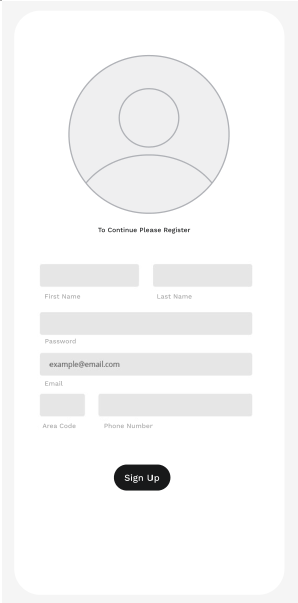
\includegraphics[width=0.2\textwidth]{register.PNG}  % 이미지 크기와 파일명 지정
    \caption{register Page}  % 이미지 캡션
\end{figure}
\subsection{Login}
Users can log in using the username and password they created during the sign-up process. When a user attempts to log in, the system verifies if the information matches the data in the database. If the credentials are incorrect, a login failure message is shown. If they are correct, the user is logged in successfully and redirected to the main page of Checkout.
\begin{figure}[H]  % 'h'는 이미지가 해당 위치에 삽입되도록 지정
    \centering  % 이미지를 중앙에 배치
    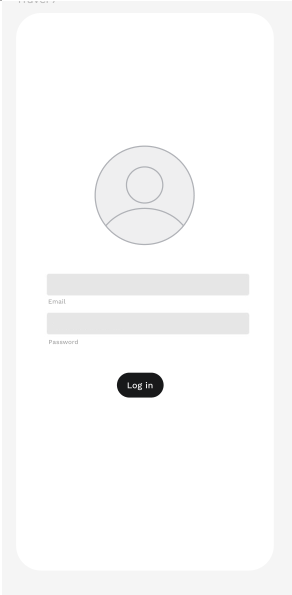
\includegraphics[width=0.2\textwidth]{login.PNG}  % 이미지 크기와 파일명 지정
    \caption{login Page}  % 이미지 캡션
\end{figure}
\subsection{Main Page}
Once logged into Checkout, the first page users will see is the main page. At the top of the Checkout main page, users can find their profile picture, name, and a welcome message. If it's the user's first time logging in, clicking "Start Checking Out" will show a tutorial for new users, explaining how to use Checkout and how to register a card.
The main page also displays recommended products, nearby markets where users can shop, and a list of recently purchased items. Users can click on a recommended product or a past purchase to see more details, including prices and purchase history.
When users click on a nearby market, the app integrates with a map application to show the route to the nearest store. The bottom navigation bar provides easy access to other pages within Checkout.
\begin{figure}[H]  % 'h'는 이미지가 해당 위치에 삽입되도록 지정
    \centering  % 이미지를 중앙에 배치
    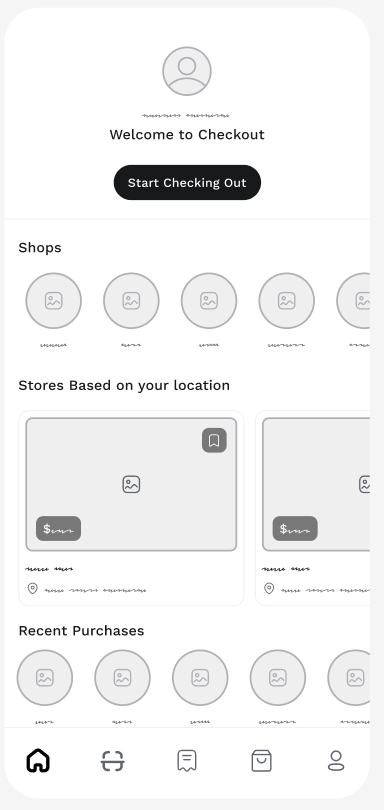
\includegraphics[width=0.2\textwidth]{main.PNG}  % 이미지 크기와 파일명 지정
    \caption{Main Page}  % 이미지 캡션
\end{figure}

\subsection{Profile}
Once logged in, users can manage their personal information on the profile page. The profile feature allows users to update payment information, addresses, and other personal details. Users can view and edit their name, email, address, and payment methods in the 'My Profile' section. Additionally, users can add or modify payment methods, allowing them to keep their profile up-to-date for a smoother experience.
If users select a payment method in their profile, they can use that payment method for checkout when they scan a barcode for payment.

\begin{figure}[H]  % 'h'는 이미지가 해당 위치에 삽입되도록 지정
    \centering  % 이미지를 중앙에 배치
    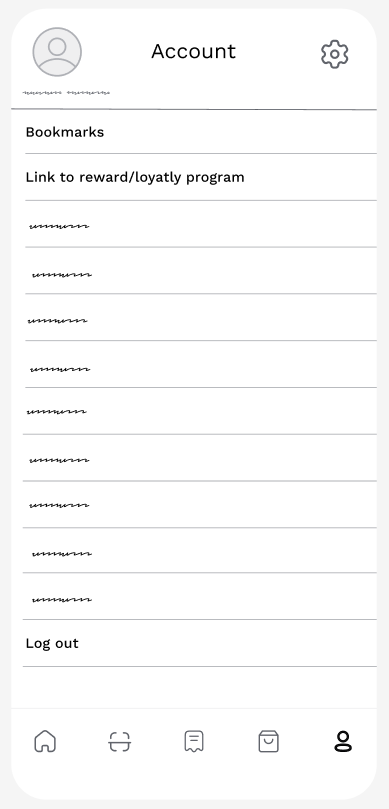
\includegraphics[width=0.2\textwidth]{account.PNG}  % 이미지 크기와 파일명 지정
    \caption{Profile Page}  % 이미지 캡션
\end{figure}


\subsection{Barcode Scan}
Users can scan the barcode of products sold in supermarkets through the Checkout mobile web app. When they click the 'Barcode Scan' button, the mobile device's camera is activated to recognize the product’s barcode. Once the barcode is scanned, the system displays real-time information about the product, such as its name, price, and stock. If users want to purchase the product, they can add it to their shopping cart.

\begin{figure}[H]  % 'h'는 이미지가 해당 위치에 삽입되도록 지정
    \centering  % 이미지를 중앙에 배치
    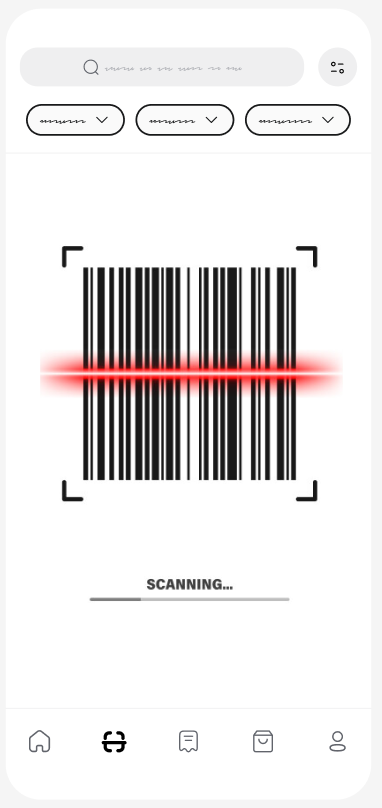
\includegraphics[width=0.2\textwidth]{barcode.PNG}  % 이미지 크기와 파일명 지정
    \caption{Barcode Scanning Page}  % 이미지 캡션
\end{figure}

\subsection{Shopping Cart}
Users can add various products to their shopping cart either by scanning barcodes or searching for items. The shopping cart allows users to see all the products they've selected at a glance. Clicking on the 'Shopping Cart' menu shows a list of items in the cart and the total price. Users can adjust the quantity of items or remove unwanted products. This feature helps users review their selections before proceeding to checkout. After reviewing the cart, users can move to the checkout page to complete the purchase.

\begin{figure}[H]  % 'h'는 이미지가 해당 위치에 삽입되도록 지정
    \centering  % 이미지를 중앙에 배치
    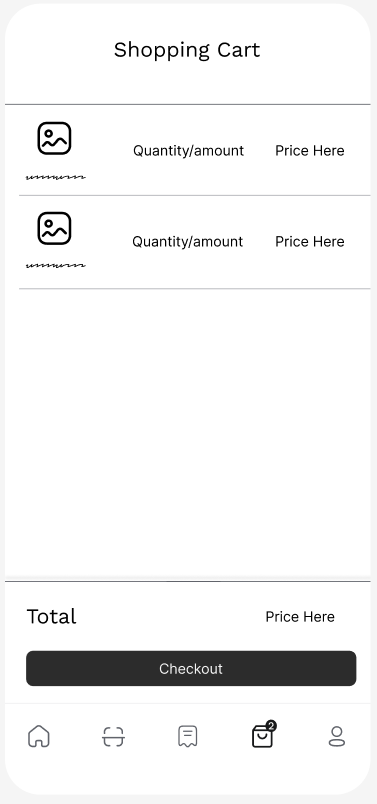
\includegraphics[width=0.2\textwidth]{shoppingcart.PNG}  % 이미지 크기와 파일명 지정
    \caption{Shoppingcart Page}  % 이미지 캡션
\end{figure}

\subsection{Payment}
Payment is the process in which users purchase the items in their shopping cart. On the payment page, users can choose from various payment methods, such as credit cards or mobile payment. After selecting the payment method (credit card, points, etc.), users enter their payment details, and the system processes the transaction. If everything is correct, the payment is completed successfully, and users receive a confirmation message along with a receipt.
If the user has made previous payments or pre-selected a payment method in their profile, the system will automatically suggest the pre-selected method.
\begin{figure}[H]  % 'h'는 이미지가 해당 위치에 삽입되도록 지정
    \centering  % 이미지를 중앙에 배치
    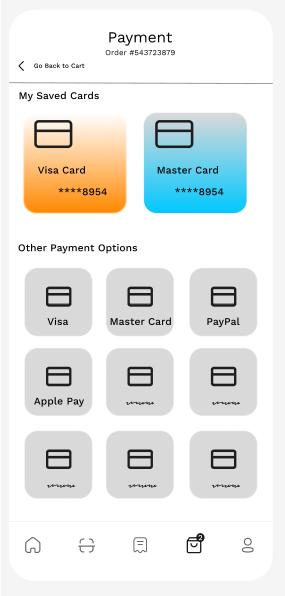
\includegraphics[width=0.2\textwidth]{payment.PNG}  % 이미지 크기와 파일명 지정
    \caption{payment Page}  % 이미지 캡션
\end{figure}
\subsection{Receipts}
Users can view their past purchases by accessing the 'My Receipts' section. The receipts include details such as the purchased items, prices, payment date, and payment method. This feature allows users to track their purchasing history and verify transaction details.

\begin{figure}[H]  % 'h'는 이미지가 해당 위치에 삽입되도록 지정
    \centering  % 이미지를 중앙에 배치
    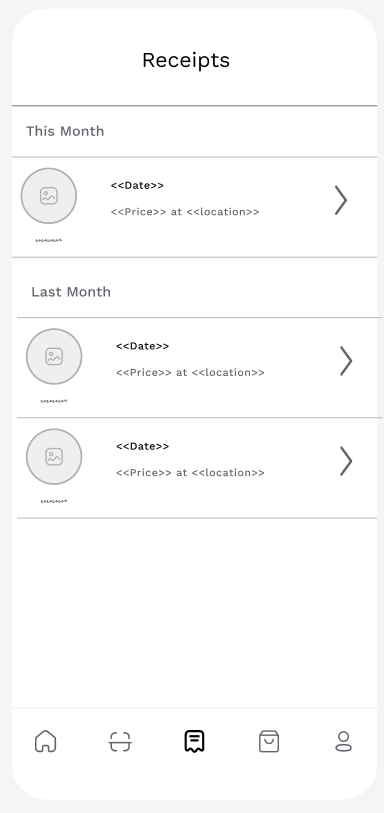
\includegraphics[width=0.2\textwidth]{receipts.PNG}  % 이미지 크기와 파일명 지정
    \caption{Receipts Page}  % 이미지 캡션
\end{figure}



\end{document}